%%%%%%%%%%%%%%%%%%%%%%%%%%%%%%%%%%%%%%%%%%%
%   Simple and elegant academic report    %
%   Copyright by Artur M. Brodzki, 2019   %
%%%%%%%%%%%%%%%%%%%%%%%%%%%%%%%%%%%%%%%%%%%

\documentclass{eiti-raport}

\usepackage[
	english,
	polish
]{babel}
\usepackage{polski}

%------------------------------------------

\begin{document}

\author{Artur M. Brodzki \\ Damian Chiliński \\ Krzysztof Sznejder}
\date{\today}
\subject{BCYB 19L}
\title{Projekt -- dokumentacja wstĘpna}
\fancyhead[L]{Brodzki, Chiliński, Sznejder}
\fancyhead[R]{BCYB 19L}

\pagenumbering{arabic}
\maketitle

%------------------------------------------
% MAIN CONTENTS
%------------------------------------------

\section{Wstęp} \label{sec:intro}
Zgodnie z przyjętym przez nas tematem, w ramach projektu napisaliśmy moduł systemu IDS/IPS Snort, wykrywający steganograficzną transmisję danych metodą tunelowania DNS. Przetestowaliśmy również jego działanie w wirtualnym środowisku, symulującym sieć korporacyjną. 

\section{Tunelowanie DNS} \label{sec:2}

\subsection{Zasada działania}
Tunelowanie DNS należy do metod steganograficznych i pozwala na prowadzenie niewidocznej dla administratorów transmisji danych, np. przesłanie na maszynę atakującego wykradzionych plików. Zasada działania opiera się na redundancji protokołu DNS. Typowy przebieg ataku z wykorzystaniem tunelowania DNS jest następujący:
\begin{enumerate}
	\item Atakujący rejestruje domenę, np. \texttt{best-malware.com} i tworzy dla niej własny serwer autorytatywny. 
	\item Atakujący instaluje złośliwe oprogramowanie na systemach ofiary, które wykrada z nich wrażliwe dane, np. hasło bankowe. 
	\item Oprogramowanie atakującego koduje uzyskane informacje jako subdomenę, np: \\  \texttt{76756C6E657261626C65.bestmalware.win} odpowiadające jej zapytanie DNS. Zapytanie na serwer atakującego, który może odebrać i zdekodować ukryte informacje. Dane można kodować zasadniczo za pomocą kodowania szesnastkowego lub base32. Wynika to ze specyfikacji protokołu DNS, który dopuszcza w zapytaniach ograniczony zestaw znaków. 
	\item Aby przeprowadzić transmisję w drugą stronę, wystarczy zakodować informację w pakiecie będącym odpowiedzią na zapytanie. Najczęściej będzie to więc pakiet typu A, choć możliwe jest kodowanie danych z użyciem każdego typu rekodu DNS. 
\end{enumerate}
Skuteczność tego ataku wynika z kluczowej roli, jaką odgrywa DNS w komunikacji internetowej. Jego zablokowanie może uniemożliwić działanie sieci, dlatego zapytania DNS bardzo rzadko są ograniczane przez administratorów, i to nawet w sieciach o restrykcyjnych wymogach bezpieczeństwa. 

\subsection{Metody wykrywania}
Aby skutecznie blokować transmisję wykorzystującą tunelowanie DNS, konieczne jest wiarygodne odróżnienie złośliwych zapytań DNS od tych prawidłowych. Stosuje się w tym celu zbiór heurystyk, opartych m.in. o:
\begin{itemize}
	\item analizę długości i entropii zapytania -- większość ,,normalnych'' domen nie przekracza kilkunastu znaków i charakteryzuje się niewielką entropią, typową dla słów pochodzących z języka naturalnego;
	\item analizę częstości -- znaczący wzrost liczby wykonywanych zapytań DNS może sugerować, że część z nich jest niepożądana;
	\item metody słownikowe -- ,,prawdziwe'' domeny zazwyczaj składają się ze słów pochodzących z języka naturalnego lub zbudowanyh na ich podstawie neologizmów;
	\item uczenie maszynowe.
\end{itemize}
W naszym projekcie zdecydowaliśmy się wykorzystać autorski algorytm uczenia maszynowego oparty na naiwnym klasyfikatorze Bayesa. Klasyfikator został nauczony na zbiorze zapytań DNS wygenerowanych i przechwyconych przez nas podczas kilku tygodni codzienniego użytkowania naszych domowych komputerów. Szczegółowy opis algorytmu znajduje sie w sekcji \ref{sec:plugin} 

\section{Scenariusz projektowy}
Zaplanowaliśmy następujący scenariusz projektowy: firma B-Cyb S.A dysponuje siecią firmową, działającą w domenie \texttt{bcyb.com}. W ramach świadczonych usług, udostępnia światu dwie usługi sieciowe, dostępne pod adresami, kolejno: \texttt{s1.bcyb.com} oraz \texttt{s1.bcyb.com}. Dostęp do firmowej sieci chroniony jest za pomocą restrykcyjnie skonfigurowanego firewalla, jak również systemu IDS/IPS Snort, filtrującego wszelki ruch przepływający przez sieć. Ponieważ firma B-Cyb obawia się ataku metodą tunelowania DNS, zakupiła od młodego zespołu specjalistów (Kant Security sp. z.o.o) dodatkowy moduł systemu Snort, mający wykrywać i blokować złośliwą transmisję. W ramach sieci firmowej została wydzielona podsieć, chroniona -- w celach testowych -- przy użyciu nowego modułu. 

Na firmowych serwerach znajduje się jednak złośliwe oprogramowanie, którego zadaniem jest przetransmitować na serwery atakującego wykradzione pliki \texttt{/etc/shadow}. Ponieważ wyprowdzenie danych poza sieć za pomocą protokołu TCP jest niemożliwe, atakujący zdecydowali się zastosować właśnie tunelowanie DNS. Podczas próby przesłania wykradzionych haseł, nowy moduł Snorta od zespołu Kant Security wykryje i zablokuje złośliwą transmisję. Natomiast podsieć chroniona za pomocą dotychczasowej wersji systemu Snort nie wykryje ataku i pozwoli na wyprowadzenie haseł na zewnątrz. 

Całość infrastruktury projektowej została zainstalowana przez nas na maszynach wirtualnych VMware i obejmuje łącznie 9 hostów, znajdujących się pod kontrolą systemu Fedora 30. Szczegółowa topologia sieci znajduje się na rys. \ref{fig:topologia}. 
\begin{figure}[!h] \centering
	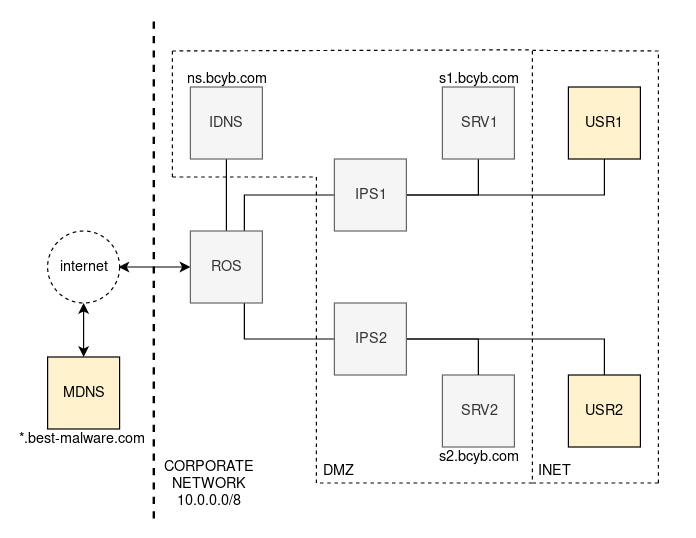
\includegraphics[width=0.9\linewidth]{img/BCYB_topologia.png}
	\caption{Schemat ideowy sieci, realizującej przyjęty scenariusz projektowy.} \label{fig:topologia}
\end{figure}
Przygotowana infrastruktura składa się z następujących urządzeń: 
\begin{enumerate}
	\item Router ROS: domyślna brama sieciowa dla sieci firmowej. Działa pod kontrolą systemu MikroTik RouterOS i obsługuje zaporę sieciową. Zapora posiada następującą konfigurację:
	\begin{enumerate}
		\item sieć firmowa (corporate network, 10.0.0.0/8) podzielona jest na strefę zdemilitaryzowaną (DMZ) oraz sieć wewnętrzną (INET);
		\item strefa zdemilitaryzowana obejmuje publicznie dostępne serwery DNS (IDNS) i HTTP (SRV1, SRV2), jak również chroniące je hosty systemu Snort (IPS1, IPS2).
		\begin{itemize}
			\item ruch wchodzący: dopuszczony jest jedynie ruch realizujący świadczone usługi, oraz ruch SSH pochodzący z sieci INET;
			\item ruch wychodzący: zabronione jest inicjowanie ruchu w obrębie DMZ, z wyjątkiem zapytań DNS oraz ruchu wychodzącego do serwerów zawierających repozytoria Fedory. Dopuszczony jest zatem jedynie ruch wymagany do pobierania aktualizacji oprogramowania systemowego;
		\end{itemize}
		\item sieć wewnętrzna obejmuje dwa komputery wyposażone w graficzny interfejs użytkownika (USR1, USR2), służące pracownikom firmy do wykonywania obowiązków służbowych, w szczególności zarządzania hostami znajdującymi się w obrębie DMZ. Zarządzanie odbywa się tylko i wyłącznie za pomocą protkołu SSH.
		\begin{itemize}
			\item ruch wchodzący: inicjowanie ruchu pochodzącego spoza sieci INET jest zabronione w każdym przypadku i na wszystkich portach;
			\item ruch wychodzący: co do zasady nie jest filtrowany, z wyjątkiem rzecz jasna ograniczeń wymuszonych przez zaporę ogniową dla ruchu wchodzącego do DMZ.
		\end{itemize}
	\end{enumerate}
	\item MDNS: maszyna atakującego. Atakujący rejestruje własną domenę \texttt{best-malware.com} i tworzy dla niej serwer autorytatywny, zainstalowany właśnie na maszynie MDNS (ang. \textit{malicious DNS}). Serwer ten stanowi punkt odbiorczy ukrytej komunikacji. 
\end{enumerate}
Z uwagi na nietrywialną złożoność wirtualizowanej infrastruktury, istotne jest określenie wymagań sprzętowych. Szczególnie ważna jest ilość pamięci operacyjnej, wymagana do działania poszczególnych hostów:
\begin{itemize}
	\item każdy z hostów posiadających graficzny interfejs użytkownika (USR1, USR2, MDNS) wymaga 2 GB pamięci RAM;
	\item hosty systemu Snort (IPS1, IPS2) wymagają do sprawnego działa po 768 MB pamięci RAM każdy;
	\item serwery HTTP (SRV1, SRV2) zajmują po 512 MB pamięci;
	\item do działania serwera DNS (IDNS) konieczne jest 512 MB, a dla routera ROS -- 256 MB pamięci RAM.
\end{itemize}
Doliczając do tego pamieć systemu gospodarza okazuje się, że dla zwirtualizowania całej wymaganej infrastruktury niezbędne jest co najmniej 12 GB pamięci operacyjnej. W praktyce będzie to zazwyczaj 16 GB. 

\section{Implementacja} \label{sec:plugin}

\subsection{Aplikacja nadawcza i odbiorcza}


\subsection{Wtyczka systemu Snort}


\section{Podsumowanie} \label{sec:summary}
Tak przygotowany scenariusz projektowy pozwoli nam na przetestowanie możliwości wykrywania tunelowania DNS z wykorzystaniem uczenia maszynowego oraz zaprezentowanie działania systemów typu IDS/IPS w praktyce. 

\end{document}
